\documentclass[10pt]{article}
\usepackage[margin=0.75in]{geometry}
\usepackage{amsmath,amssymb,booktabs,tabularx,xcolor,tcolorbox,listings,microtype}
\usepackage[hidelinks]{hyperref}
\usepackage{enumitem,tikz}
\title{\vspace{-1.5em}Distributed Policy Reasoning for Multi-Agent Systems}
\date{}
\newtcolorbox{mainbox}{colback=gray!7,colframe=black!55,boxrule=.6pt,arc=2pt}
\newtcolorbox{rulebox}{colback=gray!9,colframe=black!45,boxrule=.5pt,arc=1pt}
\lstset{basicstyle=\ttfamily\small,columns=fullflexible,keepspaces=true,
  breaklines=true,breakatwhitespace=true,comment=[l]{\%},commentstyle=\color{black!60}}
\setlist[itemize]{leftmargin=1.3em,itemsep=2pt,topsep=3pt}
\setlength{\parindent}{0pt}\setlength{\parskip}{4pt}
\begin{document}
\maketitle\vspace{-1.5em}

\section{System Overview}

We place a distributed runtime enforcement layer around a multi-agent system. The layer
combines information-flow control (IFC) and capability control. Policies and security
state are represented as Datalog facts and rules.

\begin{mainbox}
\centering
\textbf{Distributed facts + Datalog policies}\\[5pt]
\begin{tabular}{c@{\quad}c@{\quad}c@{\quad}c}
\textbf{Why} & \textbf{What-if} & \textbf{Minimal prevention} & \textbf{Speculation}\\
proof of denial & change input facts & smallest prevention & safe completion
\end{tabular}
\end{mainbox}

The same representation supports four analyses:

\begin{itemize}
\item \textbf{Why.} Ask for a proof of a fact such as \texttt{DenyReceive(A,M)}. The proof gives a derivation tree back to input facts.
\item \textbf{What-if.} Add or remove input facts, recompute the Datalog closure, and ask whether the same denial is still derived.
\item \textbf{Minimal prevention.} Find the smallest set of prior input events whose prevention removes the denial.
\item \textbf{Speculative analysis.} Search future task-relevant actions and ask whether some trace can finish the task without triggering a denial.
\end{itemize}

Facts do not need to be stored globally. Each principal stores its local facts. Messages
carry facts needed by the receiver. Policy rules can be replicated. Thus, \textbf{policy
is replicated, while state is distributed}.

\section{Running Example: Nova Budget Audit}

\subsection{Application}

\textbf{Setting.} Consider a company whose departments are represented by agents. These
agents use AI tools to organize documents and review finances, and their coordination
naturally transfers information across departmental boundaries. Access is constrained by
capabilities---for example, reviewing personnel data requires an HR review
capability---and by organization-wide policies that limit how information may accumulate
across transfers.

\textbf{Scenario.} The company is launching project Nova. Its executive board assigns
Procurement, Facility, and HR to prepare their respective budget rationales, with HR
responsible for hiring costs. Two peer auditors must jointly check all three parts.
Under the company's \emph{Three-Part Exposure Policy}, no agent other than the board may
acquire all three distinct parts of a project's rationale. Auditor A holds the
\texttt{hr\_review} capability required for the hiring part; Auditor B does not. The
auditors must therefore find a division of work that completes the audit without
violating either the capability requirement or the exposure policy. The audit is
complete once each part has been received by an authorized auditor for review.

\subsection{Tuples}

Input tuples record configuration, source labels, and runtime events; derived tuples
capture information flow, policy decisions, and audit progress. In the schemas below,
\texttt{P} is a principal, \texttt{A} an auditor, \texttt{M} a message,
\texttt{Proj} a project, \texttt{Part} a rationale part, and \texttt{Cap} a capability.
\texttt{Min} and \texttt{Mout} denote input and output messages.

Storage is either \emph{global} (shared configuration replicated across principals),
\emph{local at} a named owner, or \emph{temporary} (used while checking a proposed
receive). A message's holder is a principal that stores it; labels accompany messages
when transferred. Each auditor records its own progress, and the board collects these
progress facts to determine whether the audit is complete.

\textbf{Input tuples.}
\begin{center}\small
\setlength{\tabcolsep}{4pt}
\renewcommand{\arraystretch}{1.15}
\begin{tabularx}{\linewidth}{@{}p{0.32\linewidth} >{\raggedright\arraybackslash}p{0.10\linewidth} >{\raggedright\arraybackslash}p{0.16\linewidth} >{\raggedright\arraybackslash}X@{}}
\toprule
\textbf{Schema} & \textbf{Source} & \textbf{Storage} & \textbf{Meaning}\\
\midrule
\texttt{Auditor(A)} & config & global & \texttt{A} is authorized to act as an auditor.\\
\texttt{HasCap(P, Cap)} & config & local at \texttt{P} & \texttt{P} holds capability \texttt{Cap}.\\
\texttt{Requires(Proj, Part, Cap)} & config & global & Receiving \texttt{Part} of \texttt{Proj} requires capability \texttt{Cap}.\\
\texttt{TrustedCarry(M, Proj, Part)} & trusted app & local at sender of \texttt{M} & The trusted application attaches a sink tag to \texttt{M}, identifying \texttt{Part} of \texttt{Proj}.\\
\texttt{Sender(P, M)} & runtime & local at \texttt{P} & \texttt{P} sent message \texttt{M}.\\
\texttt{Receiver(P, M)} & runtime & local at \texttt{P} & \texttt{P} received message \texttt{M}; this event is used to track dependencies.\\
\texttt{Before(Min, Mout)} & runtime & local at \texttt{P} & \texttt{P} received \texttt{Min} before sending \texttt{Mout}.\\
\texttt{Received(P, M)} & runtime & local at \texttt{P} & \texttt{P} completed an allowed receive of \texttt{M}, updating its information state.\\
\texttt{Incoming(P, M)} & runtime & temporary & A receive of \texttt{M} by \texttt{P} is proposed and awaits a policy check.\\
\bottomrule
\end{tabularx}
\end{center}

\textbf{Derived tuples.}
\begin{center}\small
\setlength{\tabcolsep}{4pt}
\renewcommand{\arraystretch}{1.15}
\begin{tabularx}{\linewidth}{@{}p{0.32\linewidth} >{\raggedright\arraybackslash}p{0.10\linewidth} >{\raggedright\arraybackslash}p{0.16\linewidth} >{\raggedright\arraybackslash}X@{}}
\toprule
\textbf{Schema} & \textbf{Source} & \textbf{Storage} & \textbf{Meaning}\\
\midrule
\texttt{DependsOn(Mout, Min)} & derived & local at sender of \texttt{Mout} & \texttt{Mout} may depend on an earlier message \texttt{Min} received by its sender.\\
\texttt{Carries(M, Proj, Part)} & derived & local at holder of \texttt{M} & \texttt{M} carries \texttt{Part} of \texttt{Proj}, directly or through a dependency.\\
\texttt{Knows(P, Proj, Part)} & derived & local at \texttt{P} & \texttt{P} has acquired \texttt{Part} of \texttt{Proj} through an allowed receive.\\
\texttt{DenyReceive(P, M)} & derived & temporary & The proposed receive of \texttt{M} by \texttt{P} violates a policy and must be blocked.\\
\texttt{Audited(Proj, Part)} & derived & local at \texttt{A}, board & An auditor has received \texttt{Part} of \texttt{Proj} for review; the board collects this progress fact.\\
\texttt{Finished(Proj)} & derived & local at board & All three required rationale parts of \texttt{Proj} have been received by auditors for review.\\
\bottomrule
\end{tabularx}
\end{center}

\textbf{\texttt{TrustedCarry}: sink tags.} Here, a sink tag marks the project
information assigned to a department. When the board sends task message \texttt{m0}
to HR, the trusted application attaches \texttt{TrustedCarry(m0, nova, hiring)}.
This tag identifies the hiring part of Nova and seeds the IFC labels propagated to
subsequent messages; agents cannot assign trusted tags themselves.

\textbf{IFC: runtime facts and label propagation.} The messaging runtime records
\texttt{Sender} on a send, \texttt{Receiver} and \texttt{Received} on an allowed
receive, and \texttt{Before} when a received message precedes an outgoing message.
These facts establish a conservative \texttt{DependsOn} relation: an outgoing message
may depend on any earlier message received by its sender. \texttt{Carries} propagates
tags along these dependencies, while \texttt{Knows} records the parts a principal has
acquired. Thus, HR's reply to an auditor inherits the hiring tag from \texttt{m0}.

\textbf{\texttt{DenyReceive}: enforcement.} Before delivering \texttt{M} to
\texttt{P}, the runtime creates \texttt{Incoming(P, M)} and evaluates the rules.
If \texttt{DenyReceive(P, M)} is derived, delivery is blocked: \texttt{P} either lacks
a required capability or would acquire a third distinct part. Otherwise, delivery
proceeds and \texttt{Received(P, M)} is recorded. The incoming fact and denial are
temporary; a blocked receive does not update \texttt{Knows}.

\textbf{\texttt{Finished}: task completion.} \texttt{Audited(Proj, Part)} means
that an auditor has received that part for review. The board derives
\texttt{Finished(Proj)} once Procurement, Facility, and Hiring are all covered,
possibly by different auditors. This example models completion as successful delivery
for review; it does not model the auditors' subsequent budget judgments.

Only input facts are changed by analysis. Derived facts are recomputed using the
following rules.

\subsection{Datalog Rules}

\begin{rulebox}
\begin{lstlisting}
% IFC: label trusted sources and propagate labels through possible dependencies.
Carries(M, Proj, Part) :- TrustedCarry(M, Proj, Part).
DependsOn(Mout, Min) :- Receiver(P, Min), Sender(P, Mout), Before(Min, Mout).
Carries(Mout, Proj, Part) :- DependsOn(Mout, Min), Carries(Min, Proj, Part).

% Local information state after an allowed receive.
Knows(P, Proj, Part) :- Received(P, M), Carries(M, Proj, Part).

% Capability control: block a receive if a required capability is absent.
DenyReceive(P, M) :- Incoming(P, M), Carries(M, Proj, Part),
    Requires(Proj, Part, Cap), not HasCap(P, Cap).

% Three-Part Exposure Policy: block a third distinct part; the board is exempt.
DenyReceive(P, M) :- P != board, Incoming(P, M), Carries(M, Proj, C3),
    Knows(P, Proj, C1), Knows(P, Proj, C2), C1 != C2, C1 != C3, C2 != C3.

% Task progress: a part counts once an auditor has received it for review.
Audited(Proj, Part) :- Auditor(A), Received(A, M), Carries(M, Proj, Part).
Finished(Proj) :- Audited(Proj, procurement), Audited(Proj, facility), Audited(Proj, hiring).
\end{lstlisting}
\end{rulebox}

\subsection{Example State}

\textbf{Configuration.} The company has two auditors, A and B. Of the two, only A
holds \texttt{hr\_review} and may receive HR information. HR also holds this capability
to receive its own tagged task from the board.

\begin{lstlisting}
% config
Auditor(auditor_a).  Auditor(auditor_b).
HasCap(auditor_a, hr_review).
HasCap(hr, hr_review).
Requires(nova, hiring, hr_review).
\end{lstlisting}

\textbf{Messages so far.} The board has sent each department its task with the
corresponding tag: \texttt{mP0} to Procurement, \texttt{mF0} to Facility, and
\texttt{m0} to HR. Procurement and Facility have already sent their budget rationales
\texttt{mP} and \texttt{mF} to Auditor A for review. HR is now sending its hiring
rationale \texttt{mH} to A; delivery is pending a policy check. The relevant input
facts are:

\begin{lstlisting}
% Board assignments and their sink tags
TrustedCarry(mP0, nova, procurement).
TrustedCarry(mF0, nova, facility).
TrustedCarry(m0, nova, hiring).
Sender(board, mP0).  Receiver(procurement, mP0).  Received(procurement, mP0).
Sender(board, mF0).  Receiver(facility, mF0).      Received(facility, mF0).
Sender(board, m0).   Receiver(hr, m0).            Received(hr, m0).

% Department replies follow receipt of the corresponding assignments
Sender(procurement, mP).  Before(mP0, mP).
Sender(facility, mF).     Before(mF0, mF).
Sender(hr, mH).           Before(m0, mH).

% A has received Procurement and Facility; Hiring is pending
Receiver(auditor_a, mP).  Received(auditor_a, mP).
Receiver(auditor_a, mF).  Received(auditor_a, mF).
Incoming(auditor_a, mH).
\end{lstlisting}

\textbf{Derived result.} The IFC rules propagate the board's tags to the department
replies. A already knows the Procurement and Facility parts, so receiving the Hiring
part would violate the Three-Part Exposure Policy. The rules therefore derive
\texttt{DenyReceive(auditor\_a, mH)}, even though A holds \texttt{hr\_review}.
The closure includes:

\begin{lstlisting}
DependsOn(mP, mP0).  Carries(mP, nova, procurement).
DependsOn(mF, mF0).  Carries(mF, nova, facility).
DependsOn(mH, m0).   Carries(mH, nova, hiring).
Knows(auditor_a, nova, procurement).
Knows(auditor_a, nova, facility).
Audited(nova, procurement).
Audited(nova, facility).
DenyReceive(auditor_a, mH).
\end{lstlisting}

The runtime blocks \texttt{mH}, so neither \texttt{Audited(nova, hiring)} nor
\texttt{Finished(nova)} is derived.

\section{Queries}

Let \(E\) be the input facts and \(\mathrm{Closure}(E)\) their Datalog closure.
The following templates explain a denial, evaluate a proposed change, identify minimal
prevention, and synthesize a safe completion trace.

\subsection{Why}

\textbf{Question.} Why was this receive denied? A derivation tree identifies the
policy and prior events responsible, helping users understand and diagnose the denial.
\textbf{Template:} \(\operatorname{proof}_E(q)\), where \(q\) is a derived fact.
For \texttt{DenyReceive(auditor\_a, mH)}, the proof is below; \texttt{A} abbreviates
\texttt{auditor\_a}. Leaves are input facts or satisfied comparisons.

\begin{center}
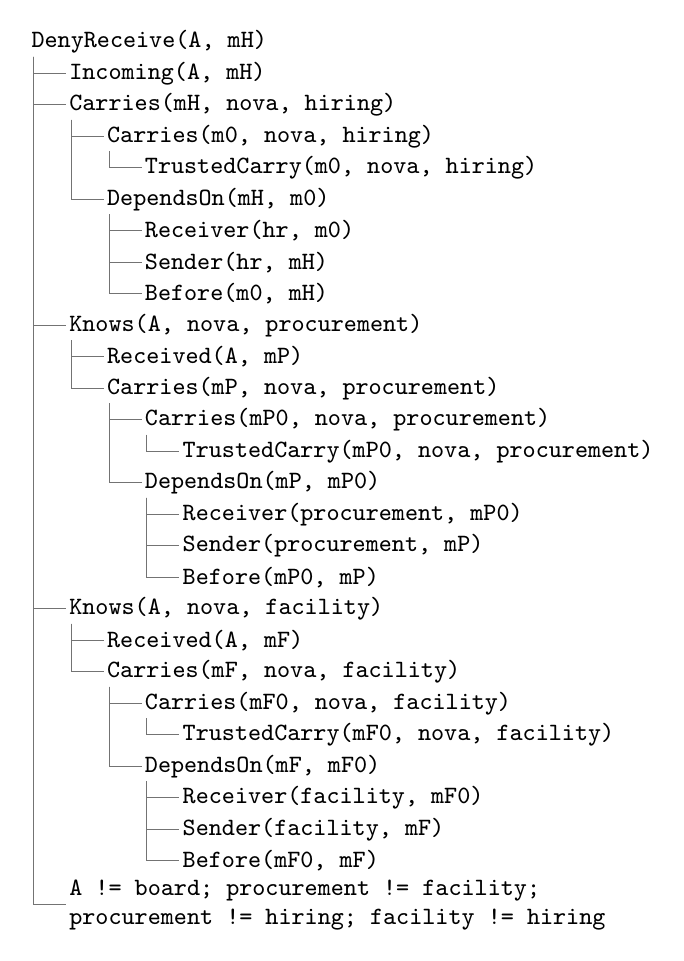
\begin{tikzpicture}[x=0.48cm,y=0.40cm,
  every node/.style={anchor=west,font=\ttfamily\small,inner sep=1pt},
  every path/.style={draw=black!55,line width=0.4pt}]
\node (n0) at (0, 0) {DenyReceive(A, mH)};
\node (n1) at (1, -1) {Incoming(A, mH)};
\node (n2) at (1, -2) {Carries(mH, nova, hiring)};
\node (n3) at (2, -3) {Carries(m0, nova, hiring)};
\node (n4) at (3, -4) {TrustedCarry(m0, nova, hiring)};
\node (n5) at (2, -5) {DependsOn(mH, m0)};
\node (n6) at (3, -6) {Receiver(hr, m0)};
\node (n7) at (3, -7) {Sender(hr, mH)};
\node (n8) at (3, -8) {Before(m0, mH)};
\node (n9) at (1, -9) {Knows(A, nova, procurement)};
\node (n10) at (2, -10) {Received(A, mP)};
\node (n11) at (2, -11) {Carries(mP, nova, procurement)};
\node (n12) at (3, -12) {Carries(mP0, nova, procurement)};
\node (n13) at (4, -13) {TrustedCarry(mP0, nova, procurement)};
\node (n14) at (3, -14) {DependsOn(mP, mP0)};
\node (n15) at (4, -15) {Receiver(procurement, mP0)};
\node (n16) at (4, -16) {Sender(procurement, mP)};
\node (n17) at (4, -17) {Before(mP0, mP)};
\node (n18) at (1, -18) {Knows(A, nova, facility)};
\node (n19) at (2, -19) {Received(A, mF)};
\node (n20) at (2, -20) {Carries(mF, nova, facility)};
\node (n21) at (3, -21) {Carries(mF0, nova, facility)};
\node (n22) at (4, -22) {TrustedCarry(mF0, nova, facility)};
\node (n23) at (3, -23) {DependsOn(mF, mF0)};
\node (n24) at (4, -24) {Receiver(facility, mF0)};
\node (n25) at (4, -25) {Sender(facility, mF)};
\node (n26) at (4, -26) {Before(mF0, mF)};
\node (n27) at (1, -27.4) {\shortstack[l]{A != board; procurement != facility;\\procurement != hiring; facility != hiring}};
\draw (n0.south west) ++(0.14,0) |- (n1.west);
\draw (n0.south west) ++(0.14,0) |- (n2.west);
\draw (n2.south west) ++(0.14,0) |- (n3.west);
\draw (n3.south west) ++(0.14,0) |- (n4.west);
\draw (n2.south west) ++(0.14,0) |- (n5.west);
\draw (n5.south west) ++(0.14,0) |- (n6.west);
\draw (n5.south west) ++(0.14,0) |- (n7.west);
\draw (n5.south west) ++(0.14,0) |- (n8.west);
\draw (n0.south west) ++(0.14,0) |- (n9.west);
\draw (n9.south west) ++(0.14,0) |- (n10.west);
\draw (n9.south west) ++(0.14,0) |- (n11.west);
\draw (n11.south west) ++(0.14,0) |- (n12.west);
\draw (n12.south west) ++(0.14,0) |- (n13.west);
\draw (n11.south west) ++(0.14,0) |- (n14.west);
\draw (n14.south west) ++(0.14,0) |- (n15.west);
\draw (n14.south west) ++(0.14,0) |- (n16.west);
\draw (n14.south west) ++(0.14,0) |- (n17.west);
\draw (n0.south west) ++(0.14,0) |- (n18.west);
\draw (n18.south west) ++(0.14,0) |- (n19.west);
\draw (n18.south west) ++(0.14,0) |- (n20.west);
\draw (n20.south west) ++(0.14,0) |- (n21.west);
\draw (n21.south west) ++(0.14,0) |- (n22.west);
\draw (n20.south west) ++(0.14,0) |- (n23.west);
\draw (n23.south west) ++(0.14,0) |- (n24.west);
\draw (n23.south west) ++(0.14,0) |- (n25.west);
\draw (n23.south west) ++(0.14,0) |- (n26.west);
\draw (n0.south west) ++(0.14,0) |- (n27.west);
\end{tikzpicture}
\end{center}

\subsection{What-if}

\textbf{Question.} Would a proposed change remove the denial? This checks a specific
counterfactual before changing the system. \textbf{Template:} specify input facts to
\texttt{REMOVE}, facts to \texttt{ADD}, and a fact to \texttt{QUERY}; evaluate the query
in \(\mathrm{Closure}((E\setminus R)\cup A)\).
If A had not received Facility:

\begin{lstlisting}
REMOVE { Receiver(auditor_a, mF), Received(auditor_a, mF) }
ADD    { }
QUERY  DenyReceive(auditor_a, mH)
RESULT false
\end{lstlisting}

Both records of the Facility receive are removed. A would then acquire only a second
part and holds the required HR review capability, so neither denial rule applies.

\subsection{Minimal Prevention}

\textbf{Question.} What is the smallest set of earlier events whose prevention would
have avoided this denial? This identifies minimal interventions without requiring the
user to guess a counterfactual. \textbf{Template:} given input state \(E\), a denial
\(q\), and a configurable \emph{preventable events set} \(\mathcal{P}\), return a
minimum-cardinality subset \(\Delta\subseteq\mathcal{P}\) whose prevention removes \(q\).

Each event \(e\) has input records \(R(e)\); preventing it removes those records and
recomputes derived facts. In this example, only A's two earlier audit receives are
preventable. Configuration, board assignments, and the pending Hiring receive remain
fixed:

\begin{lstlisting}
PREVENTABLE EVENTS P = { eP, eF }
R(eP) = { Receiver(auditor_a, mP), Received(auditor_a, mP) }
R(eF) = { Receiver(auditor_a, mF), Received(auditor_a, mF) }
QUERY q = DenyReceive(auditor_a, mH)
\end{lstlisting}

The objective is
\[
\underset{\Delta\subseteq\mathcal{P}}{\operatorname{minimize}}\; |\Delta|
\qquad\text{subject to}\qquad
q\notin\mathrm{Closure}\!\left(E\setminus\bigcup_{e\in\Delta}R(e)\right).
\]
Enumerating subsets of \(\mathcal{P}\) gives two minimum solutions:
\(\Delta=\{e_P\}\) or \(\Delta=\{e_F\}\), where \(e_P\) and \(e_F\) denote
\texttt{eP} and \texttt{eF}. Preventing either receive avoids the third-part denial.
This objective removes the specified denial; it does not require the audit to finish.

\subsection{Speculative Dead-End Analysis}

\textbf{Question.} Can the remaining work finish without any denied receive, and which
next actions preserve that possibility? A locally allowed action may still leave the
task impossible to complete. \textbf{Template:} given a starting state \(E_0\), a goal
\(G\), and a configurable action set \(\mathcal{A}\), synthesize a finite trace
\(\pi=(a_1,\ldots,a_k)\) such that every receive is allowed and
\(G\in\mathrm{Closure}(E_k)\). A state is a dead end if no such trace exists within
the configured action set.

Here, start earlier: A has received only Procurement, while Facility and Hiring remain
unaudited. The goal is \texttt{Finished(nova)}. The configured actions deliver each
department's tagged rationale to either auditor:

\begin{lstlisting}
GOAL Finished(nova)
ACTIONS {
    Procurement -> A, Procurement -> B,
    Facility    -> A, Facility    -> B,
    Hiring      -> A, Hiring      -> B
}
\end{lstlisting}

The action set is supplied by the application and can be changed. In this task model,
only department-to-auditor deliveries can add the missing \texttt{Audited} facts needed
for \texttt{Finished}, so other sends are excluded. At each state, actions for already
audited parts are also omitted: every remaining allowed action makes progress toward
the goal. Capability grants, policy changes, and other workflows are outside this
configured search, so a dead-end result is relative to these choices.

For each candidate action, the analyzer supplies the message's propagated labels and a
hypothetical \texttt{Incoming} fact. A derived \texttt{DenyReceive} rejects the action;
otherwise, the successor records the allowed receive and recomputes the closure.
The search returns a completion trace, or \texttt{NONE} if none exists:

\begin{rulebox}
\begin{lstlisting}
COMPLETE(E, G, Actions):
    if G in Closure(E): return []
    for a in ProgressActions(E, Actions):
        if Denied(E, a): continue
        E_next = HypotheticalReceive(E, a)
        tail = COMPLETE(E_next, G, Actions)
        if tail is not NONE: return [a] + tail
    return NONE
\end{lstlisting}
\end{rulebox}

This search terminates because each step audits a previously unaudited part, and Nova
has only three parts. Sending Facility to A is allowed immediately, but leaves Hiring
with no legal receiver: A would acquire a third part, and B lacks \texttt{hr\_review}.
That successor is a dead end. Sending Facility to B instead admits the completion
trace \texttt{[Facility -> B, Hiring -> A]}, which derives \texttt{Finished(nova)}
without a denial.

\end{document}
